Deep neural network has shown its great power on large scale image recognition tasks, but sometimes it is more important to get good representation of the image rather than learning the complex hierarchical representations\cite{CoatesNL11}. The main drawback of learning the high-level representation for many systems is their complexity and expense. Moreover, the multi hyper-parameters of these algorithms which would affect the performance significantly require many prior knowledge as well as computational expensive validation to determine their values. Since the unsupervised pre-training can learn some important representations,  as one of the most basic and fast unsupervised learning strategy, K-Means can also learn the representation well through a self-taught procedure. For a K-Means algorithm, the only parameter $K$ decides the number of the centroids that the data can generate. As a mature algorithms, there are many techniques that can accelerate its convergence\cite{pelleg1999accelerating}\cite{pelleg2000x}\cite{gibou2002fast}. K-Means has been defined as a successful method to learn features
from images by computer vision researchers. The term of "bag of features" is very popular in computer vision communities\cite{csurka2004visual}\cite{lazebnik2006beyond}.

In our system, the feature representation is learned as the following steps:
\begin{enumerate}
  \item learning the bag of features from sub-patches with K-Means to get a low level features.
  \item combining the low level features to generate a higher-level features.
  \item mapping the image to the feature space and do the classification.
\end{enumerate}
The concept of an ROIs (region of interests) is commonly used in many application areas especially in medical image (magnetic resonance imaging, MRI) process\cite{desikan2006automated}. It is based on a simple and intuitive hypothesis: there could always be some objects or features that appear in some certain location of the image which can be used to identify the image. This hypothesis can be applied to many other real world applications such as hand digital recognitions.
\begin{figure}
  \centering
  % Requires \usepackage{graphicx}
  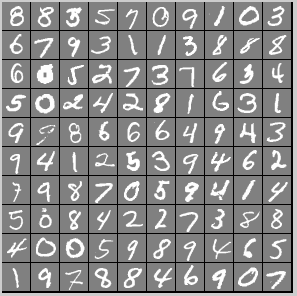
\includegraphics[scale = 1]{fig/MNST.png}\\
  \caption{The first 100 images in MNST dataset}
\end{figure}

\subsection{learning the patches with K-Means}
The classic K-means clustering algorithm finds cluster centroids that minimize the distance between data points and the nearest centroid.Also called
"vector quantization", K-means can be viewed as a way of constructing a dictionary $D \in {R^{n \times k}}$ of k vectors so that a data vector $x_(i) in R_n, i = 1...;m$
can be mapped to a code vector that minimizes the error in reconstruction.
\begin{equation}\label{}
  \mathop {\min }\limits_S {\text{ }}\sum\limits_i ^k{\sum\limits_{{x_j} \in {S_i}} {{{\left\| {{x_j} - {\mu _i}} \right\|}^2}} }
\end{equation}
$\mu_i$  is the mean of $S_i$.

In our task, the images are $28 \times 28$ pixels grayscale images and we use $14 \times 14$ pixels patch presented as a 196 pixel intensities for the K-means to learn the features. We select 12 location to generate the patches (shown in \figref{location}). For each location we use K-means to get 100 centroids with \emph{K-means++} which can avoid the sometimes poor clusterings found by the standard k-means algorithm.\cite{arthur2007k}.
\begin{figure}
  \centering
  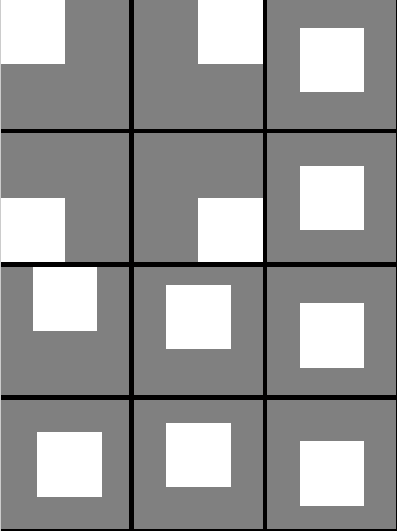
\includegraphics[scale=.5]{fig/patch_location.png}\\
  \caption{The 12 locations of the patch}
\end{figure}\label{location}

\begin{figure}[t]
  \centering
  \subfloat[Location of the patch in original image]{
  \raisebox{15mm}
    {
\includegraphics[scale=.8]{fig/patch1.png}}
  }
  \qquad
  \subfloat[100 Centroids of this location]{
     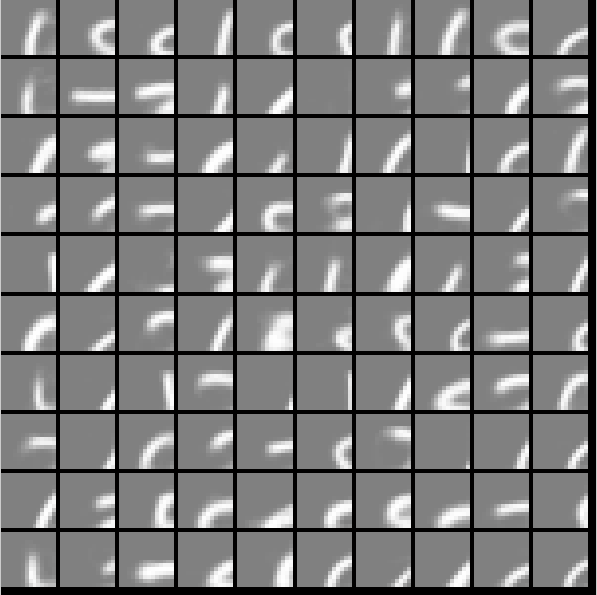
\includegraphics[scale=.5]{fig/c1.png}
  }
  \caption{The Centroids for location 1.}
\end{figure}


\subsection{Patch Combination}
The initial intuition of patch combination is the hierarchical feature representation. The higher level features can be presented as the combination of the lower ones. The idea of sparse coding is also to use the lower level features to represent the higher ones with linear combination\cite{GrosseRKN07}. In sparse coding, the lower features are linearly overlapped on each other to generate the complex higher level ones and the dimensions of the new feature will never change. In our task,  we don't overlap the lower ones. Alternatively, as we already know the specific location of each patch in the original image, we can combine the lower features in different locations of the image and generate the higher ones.
\begin{figure}[h]
  \centering
  % Requires \usepackage{graphicx}
  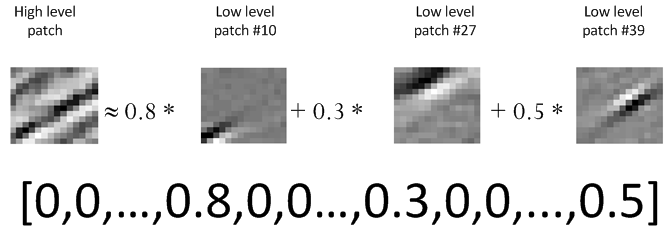
\includegraphics[scale = .75]{fig/sparsecoding.png}\\
  \caption{The idea of sparse coding}
\end{figure}
\begin{figure}[h]
  \centering
  % Requires \usepackage{graphicx}
  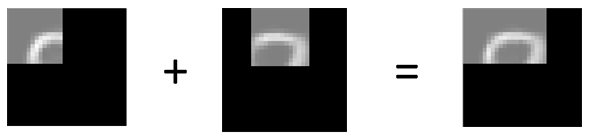
\includegraphics[scale = .75]{fig/patchcombine.png}\\\
  \caption{The combination of patches in different locations of the image}
\end{figure}
When combining two low level features, the most simple method could be just consider the number of the common instances that appear in both. If they have a lot of instances in common, these two low level features can be combined as a new one. Consider the image dataset $D$ has $n$ instances $(D \in R^{n \times m})$ and for each candidate patch location $l$ which are clustered into $k$ clusters, $D$ can be represented as a sparse binary matrix $D^l \in R^{n \times k}$
\begin{equation}
  D^l _{i,j}= \left\{ \begin{gathered}
  {D^l_{i,j}} = 1,{\text{ if }}{D_i} \in {\text{cluster }}j \hfill \\
  {D^l_{i,j}} = 0,{\text{ if }}{D_i} \notin {\text{cluster }}j \hfill \\
\end{gathered}  \right.
\end{equation}
When we have two patch location candidates $l_1$ and $l_2$, $C^{com}=D^{l_1} \times {D^{l_2}}^T$ and $C^{com}_{i,j}$ denotes the number of the common instances that for $i_{th}$ cluster in $l_1$ and $j_{th}$ cluster in $l_2$. However, $C^{com}$ just indicates how many instances that both of these two clusters hit but ignores the how many instances actually there are in each of the clusters. For instance, cluster A and cluster B has 100 and 200 instances respectively and $C^{com}_{A,B}=100$, if cluster C and cluster D has 1000 and 800 instances respectively and $C^{com}_{C,D}=150$, it is hard to say that the combination of C and D is better than A and B.

Alternatively, to evaluate the quality of the combination of the $k_1$ cluster in $l_1$ and the $k_2$ cluster in $l_2$, we can get the $k_1$ and $k_2$ column of the sparse matrix $D^{l_1}$ and $D^{l_2}$ and get the confusion matrix as Table \ref{confusion}. In the method we mentioned above, the \# of instance in common just take the \emph{True Positive} into account while ignoring the impact of \emph{False Positive} and \emph{False Negative}. In pattern recognition, the concept of \emph{precision} and \emph{recall} which are defined as Equation (\ref{eq:pr}),can solve this problem\cite{powers2011evaluation}. From Table \ref{confusion}, the precision and recall are switched when we switch cluster $i$ and $j$. But we want some score which can satisfy $score(i,j) = score(j,i)$.
Here precision and recall refer to the fraction of the "hit" in both clusters. And \emph{F-measure} can take both recall and precision into account which is defined as Equation(\ref{eq:fm}). If we set $\beta = 1$, $F_1$ is symmetric for precision and recall. So we can get $F_1(i,j) = F_1(j,i)$. For each pair of location candidates $l_1$ and $l_2$, each of which consists of $k$ centroids, we can get a $k \times k$ symmetric matrix $ComScore=\left\{ComScore_{i,j}|ComScore_{i,j}=F_1(i,j),i,j=1,2,...,k \right\}$ where $ComScore_{i,j}$ indicates the F-measure for the combination of $i_{th}$ cluster in $l_1$ and the $j_{th}$ cluster in $l_2$. If $ComScore_{i,j}$ is great than some threshold $\theta$, then the new location $l_1+l_2$ will include the centroid $k_1+k_2$ and the membership of the new centriod would be the instances in both of these two clusters.
\begin{equation}\label{eq:pr}
  \begin{gathered}
  precision = \frac{{TP}}{{TP + FP}} \hfill \\
  recall = \frac{{TP}}{{TP + FN}} \hfill \\
\end{gathered}
\end{equation}

\begin{equation}\label{eq:fm}
 {F_\beta } = \left( {1 + {\beta ^2}} \right)\frac{{precision \cdot recall}}{{\left( {{\beta ^2} \cdot precision} \right) + recall}}
\end{equation}
\begin{table}[H]
  \centering
  \begin{tabular}{ |l | p{5cm}| p{5cm}|}
  \hline
    & j & $\neg$ j \\
    \hline
  i& \# of instances both has $i_{th}$ and $ j_{th}$ feature (True Positive)& \# of instances only has $i_{th}$ feature (False Positive)\\
   \hline
  $\neg$ i & \# of instances only has $j_{th}$ feature (False Negative) & \# of instances has neither $i_{th}$ nor $ j_{th}$ feature (True Negative)\\
  \hline
\end{tabular}
  \caption{Confusion Matrix for cluster $i$ and cluster $j$}\label{confusion}
\end{table}
From \figref{fig:comb} we can see that, the combination of the patch location are very flexible, which can create some ambiguous shapes of patches that can describe some important features in the image. Compared with the conventional convolutionary method, which requires large computing and is very sensitive to the size of the kernels, our method can generate kernels with any size and any shape from some small lower patches.
\begin{figure}[h]
 \centering
\begin{tabular}{c}
   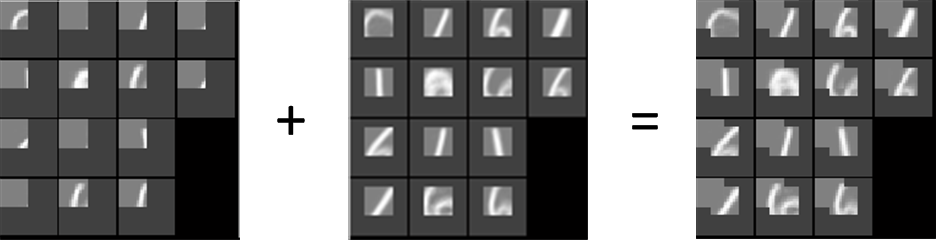
\includegraphics[scale = .5]{fig/combine2.png}\\
   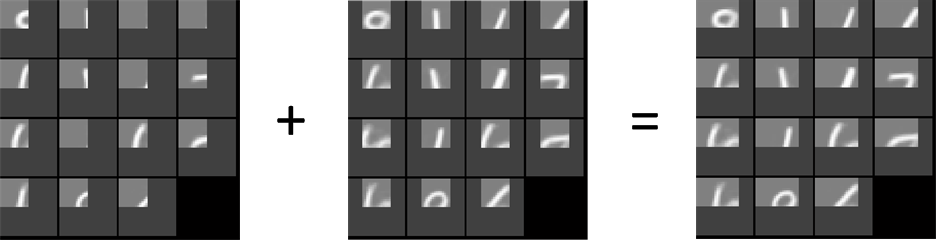
\includegraphics[scale = .5]{fig/combine.png}\\
\end{tabular}
  \caption{Successfully combined patches}\label{fig:comb}
\end{figure}

\subsection{Patch Ranking}

From the patch combination, for a particular threshold $\theta$, we can get many features with ambiguous size and shape. These centroids, generated from either k-means (low level features) or combination of the lower feature(high level features), are used as the template for the image representation. But too many features can lead the algorithm to be very slow as well as some duplicate features. Therefore, some less informative centroids (templates) should be removed. These centroids should be redundant, duplicate or irrelevant. Here both the supervised and unsupervised patch ranking techniques can be used. Unsupervised patch ranking is used to eliminate the centroids whose clusters are either too sparse or too small. Supervised patch ranking is used to eliminate those centroids that are duplicate which can no longer provide extra information after the class label is introduced.

\begin{figure}[t]
  \centering
  \subfloat[Clusters with the same centroids but different $\mu$]{   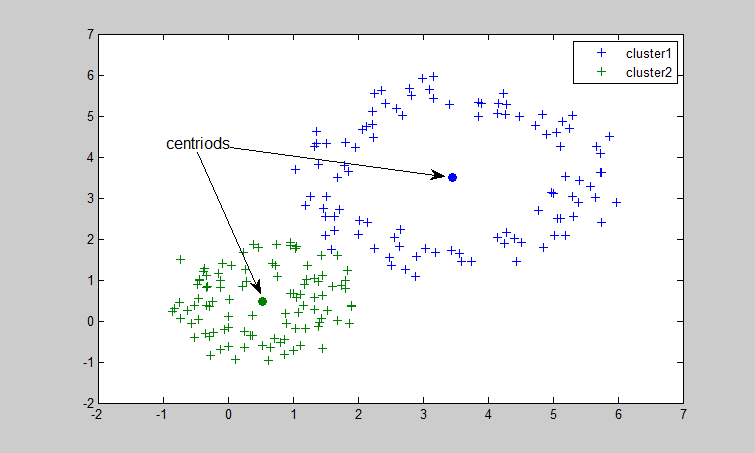
\includegraphics[scale = .5]{fig/cluster_cmp1.png}}
  \\
   \subfloat[Clusters with the almost the same centroids but different size]{ \label{fig:cmp2}  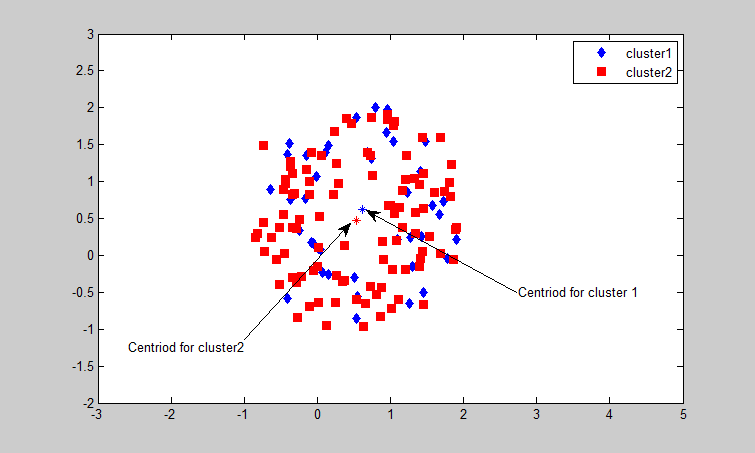
\includegraphics[scale = .5]{fig/cluster_cmp2.png}}
  \caption{Two situation to evaluate the cluster/centroid}
\end{figure}
\subsubsection{Unsupervised Patch Ranking}

In all these centroids we get from patch combination , some of the lower ones would be less informative after they are successfully combined to generate the higher ones. For instance, if $k_1$ centroid in $l_1$ and  $k_2$ centroid in $l_2$ have identical membership in the original image set and they can definitely generate a higher centroid $k_3$ in location $l_3$ which will contain identical membership as $k_1$ and $k_2$. In this situation,  $k_1$ and $k_2$ would be the duplicate patches as the higher level centroid $k_3$ can provide the information as much as them. However, we can not simply assume that all the lower features are less informative than the higher ones. Normally lower clusters can have more instances belong to compared with higher ones.In \figref{fig:cmp2}, cluster 1 has 40 instances while cluster 2 has 100 instances. The distance of them are very near and they all have the almost the same average distances to the centroid. Here, the cluster 2 is more general and its centroid can better describe the feature of its member. A more complicated situation could be the comparison of the centroids with different shape. Here we introduce the following equation for evaluation of the centroid.
\begin{equation}\label{eq:rank}
  Dist(x,C) = \underbrace {\frac{1}{n}\sum\limits_{i = 1,{x_i} \in C}^n {\frac{{{x_i} \times C}}{{\left| {{x_i}} \right|\left| C \right|}}} }_{mean{\text{ cosine similarity}}} + \alpha  \cdot  \underbrace {\log \left( n \right)*\log ({C_{size}})}_{\begin{subarray}{c}
  {\text{size of the cluster and }} \\
  {\text{size of the centroid}}
\end{subarray} }
\end{equation}
Here, the $x$ is all the cluster members and $C$ is their centroid. $n$ denotes the size of the cluster and the $C_{size}$ is the size of the number of pixels of the centroid $C$ which is positive proportional to the level of the feature. The first part of Equation (\ref{eq:rank}) is the mean cosine distance of the cluster members to the centroid which describe the similarity among the cluster members. Cosine Similarity is to calculate the orientation of two vectors instead of the magnitude which is less sensitive to the size of the pixels evaluating the centroids with different number of pixels.
The second part is for normalization which involves the size of the cluster and the size of the centroid. Our intuition is that if two clusters have the same similarity among their members, the higher level feature/centroid and the cluster with more instances has a higher rank.

Even though, there are many mature techniques for cluster analysis (like Davies–Bouldin index\cite{davies1979cluster}, Dunn index\cite{dunn1973fuzzy}, etc), which is the essence method to obtain the templates,we still want to use the most basic criterion, mean distance to the centroid, as our fundamental criterion. The unsupervised ranking is used here as the prior method of the supervised one which can be more sophisticate and useful than the unsupervised one. And it is better to use to unsupervised ranking before the supervised one as there could be too centroids, if we can't eliminate some of them with the fast unsupervised one, it could be very slow for the supervised ranking method to deal with a lot of centroids.

\subsubsection{Supervised Patch Ranking}
After eliminating the sparse centroids, the supervised patch ranking can eliminate more duplicate and irrelevant centriods to improve the results. This procedure can be considered as the feature selection which is very important in the pattern recognition system. Our ultimate goal is to improve the classification result after the patch ranking. However, without supervised ranking, there could be some embarrassing situations, like in \figref{fig:unsup_100}. For the classification of digital number 1 and 3, some important features for both of the classes should be found before the final classification. But after the unsupervised ranking, most of the features with higher rank are for the digital 1. There is just one feature (in red box) for digital 3. Even though this matters a little for the binary situation, this could be a serious problem for multi-class problem as some of the classes may not get enough features to be distinguished. So the goal of the supervised ranking is to found those centroids that can represent each of the classes and eliminate the redundant and irrelevant ones.
\begin{figure}[H]
  \centering
  % Requires \usepackage{graphicx}
  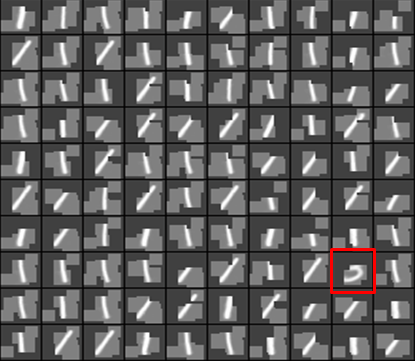
\includegraphics[scale = .5]{fig/100_unsup.png}\\
  \caption{Top 100 unsupervised ranking centroids for classification of digital number 1 and 3}\label{fig:unsup_100}
\end{figure}
\textbf{Significant Test}
The typical supervised feature selection can be formulated like: given the dataset $D$ that contains $N$ samples with $M$ features $F={f_i, i=1,...,M}$ as well as the target class $c$, feature selection is to find the optimal subspace $m$ of the $M-dimension$ that can best characterized $c$. As there could be $2^M$ candidates, it is really hard to search the space exhaustively. Here the $optimal$ leads to the $minimal classification error$ which is to find the maximal statistical dependency of the target class $c$ on the data distribution in the subspace $R^m$.  From this, the most simple method could be the significant test for each feature with specific target class $c$.
\begin{figure}[H]
  \centering
  % Requires \usepackage{graphicx}
  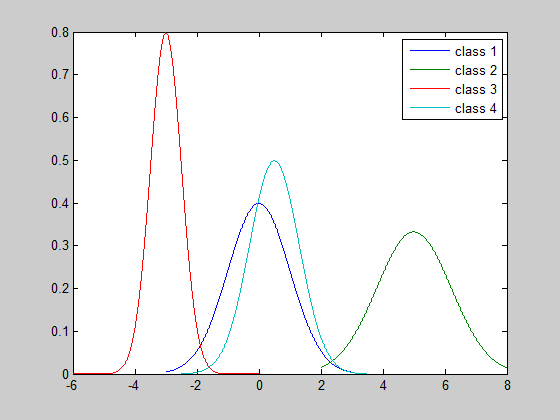
\includegraphics[scale = .75]{fig/sign.png}\\
  \caption{Significant test for feature selection for the 4 classes situation for specific feature $f_i$}\label{fig:sign}
\end{figure}
From \figref{fig:sign} it is easy to find that the class 1 and class 4 are almost overlapped and with some significant test (like $t-test$), class 1 and class 4 can not be distinguished with the feature $f_i$. Still, there should be some criterion for the supervised ranking with significant test:
\begin{enumerate}
  \item Features that are significantly distinguishable for all classes should be rank the highest. These features are global features that can be used to "vote accept" for the every class.
  \item Features that are significantly distinguishable for more classes should be rank higher. These features are local feature for specific one or more classes and they can "vote reject" for at least one class.
  \item Features that are not significantly distinguishable for all classes are the redundant and irrelevant ones which should be eliminated and rank the lowest.
\end{enumerate}

\textbf{Mutual Information}
The significant test can check the dependency of target class on the data distribution for some features. It is easy to check for a single feature, as we want to find the best $m$ features and the final performance is determined by the joint result of the features, the significant test can't solve this well. In information theory, the mutual information of two random variables is a measure of the mutual dependence of the two random variables. Given two random variables $X$ and $Y$, their mutual information is defined in terms of their probabilistic density functions $p(x)$, $p(y)$, and $p(x,y)$:
\begin{equation}\label{mutualinfor}
  I(X,Y) = \int_Y {\int_X {p(x,y)\log \frac{{p(x,y)}}{{p(x)p(y)}}dx} dy}
\end{equation}
Intuitively, mutual information measures the information that X and Y share: it measures how much knowing one of these variables reduces uncertainty about the other. For example, if X and Y are independent, then knowing X does not give any information about Y and vice versa, so their mutual information is zero. At the other extreme, if X and Y are identical then all information conveyed by X is shared with Y: knowing X determines the value of Y and vice versa. As a result, in the case of identity the mutual information is the same as the uncertainty contained in Y (or X) alone, namely the entropy of Y (or X: clearly if X and Y are identical they have equal entropy) \cite{mackay2003information}. Here Y can be the target class $c$ and X can be any dimension (feature) in the $M-dimension$ space. For each individual feature, $I(X,c)$ reflects the dependency of the class on the feature X. the top $m$ $I(X,c)$ in descending order are the features to be selected.

It is clear that in neither significant test nor mutual information criterion, the top $m$ selected features are not necessarily to be the "$m$ best features" as the relationship between the features is not considered. To obtain the "$m$ best features", it is to search the best $m$ combination of the features which can be applied in two opposite directions with the filter: forward  and the backward selections \cite{peng2005feature}.
\begin{enumerate}
  \item The forward selection tries to select a subset of $m$ features from $M$ in an incremental way. At first we set the candidate set $S_{cand}=M$ and $S_{sel} = \emptyset$ as well as the criterion for the selection $Cr$. For each iteration, we pick up a feature $x$ from $S_{cand}$ and evaluate $Cr(x+S_{sel})$. The best $x_{best}$ will be add into $S_{sel}$ as well as remove from $S_{cand}$. This would stop in $m$ iterations.
  \item The backward selection manners from the other direction. It first set $S_{sel} = M$ and subtract the irrelevant features from it until stop. The backward selection is often used to select a large subset which is obviously faster than the forward selection.
\end{enumerate}

It is worthy to mention that normally the result of the forward selection is not the same as the one with backward selection for the same problem and the same settings. As both of them are following a gradient descent manner, for most of the real world problems which have many local minimum, it is rare for both of them to meet at the same terminal for the same problem.

\subsection{Encoding with the centroids}
After obtaining all these centroids, the more important thing is to map the original image into the new feature space according to the centroids which essentially turns into the similarity metric problem. The intuition of the encoding is that for images $I_1$, $I_2$ and the template $t$, we have to find a similarity function, called distance function, $D(x,y)$ must satisfy that if $I_1$ is more similar to $t$ than $I_2$, $D(I_1,t) > D(I_2,t)$. However, similarity is much complicated when described in the mathematical function than it looks. When dealing with similarity in our human brain for the images, we can do the shifting, scaling, rotation and other geometric transformation in parallel and get the result almost on real time. For computer vision researchers, each of these transformation is applying a kernel matrix on the original image and combine each possible results together. In practical, even though there could be infinite possible combinations, we can set some fix interval for each of the transformation, so each transformation can be divided into several intervals which is still a cost computation process.

However, it is still widely believed that the simplest method is the most practical one. Complexity can lead to uncertainty. Therefore, original Euclidean Distance is still the most popular method as the similarity metric. Even though, it is a naive method which only depends on the intensity of the pixels and is very sensitive to the deformation. There are many variance of it such as\cite{buades2005non}\cite{maurer2003linear}:
 \begin{equation}\label{eq:edv}
   d({I_1},{I_2}) = {\left( {{I_1} - {I_2}} \right)^T}G\left( {{I_1} - {I_2}} \right)
 \end{equation}
This can be considered as the weighted Euclidean Distance for images $I_1$ and $I_2$. The weight matrix $G$ is computed by the pixel dependency of the pixels in both images. As the weight matrix can be defined by users, it can be more flexible. For instance, if $G$ is computed by the coefficient of the pixels in the image, the weighted Euclidean Distance can fit small deformation. After adding the weight matrix, the weighted Euclidean Distance can be less sensitive.

Neural network is considered as the efficient encoder for many researchers\cite{rehn2007network}\cite{Srivastava13}\cite{Hinton12}. RBM, as the one layer neural network can be the efficient encoder. The free energy of the RBM can be used to determine whether the model is overfitting as well as for discrimination directly.The free energy is defined as:
\begin{equation}\label{eq:fe}
  F(v) =  - \sum\limits_i {{v_i}{a_i}}  - \sum\limits_j {\log (1 + {e^{{x_i}}})}
\end{equation}
 The parameters $v_i$ and $a_i$ here are the same as the ones defined in Equation (\ref{eq:engery}) and ${x_j} = {b_j} + \sum\limits_i {{v_i}{w_{ij}}}$.

 If the model is not overfitting at all, the free energy should be about the same on the training and validation set\cite{Hinton12}. According to this, if the model is not overfitting, the free energy can be used to determine whether the test sample is similar to the data in training set. For each of the cluster, we can build a RBM and use the its free energy to encode each individual sample.
\begin{figure}
  \centering
  % Requires \usepackage{graphicx}
  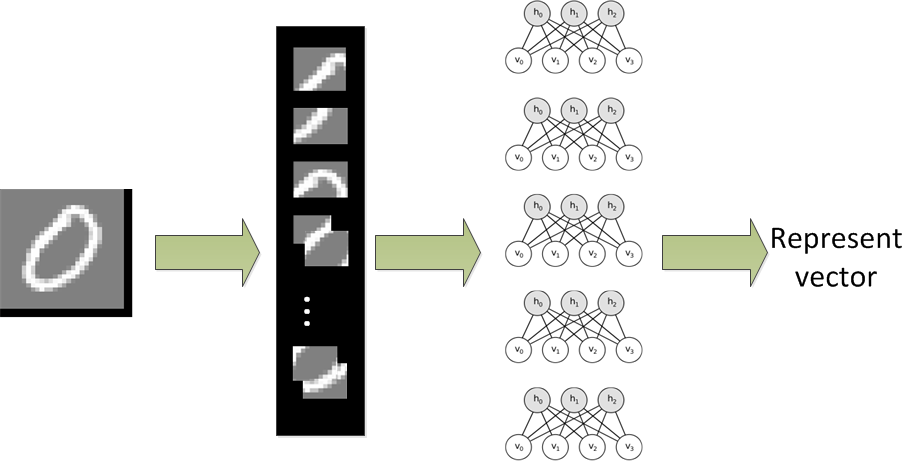
\includegraphics[scale = .5]{fig/RBM_encoder.png}\\
  \caption{Use free energy of RBMs as the encoder}
\end{figure}

 Overall, no matter the weighted Euclidean Distance or the RBM encoder with free energy, they are trying to find the proper metric to evaluate the similarity for images. SIFT can detect the same objects in two images and get rid of the affects of rotation, scaling and lighting condition \cite{lowe1999object}. However SIFT can only detect identical objects in the two images. When the two objects are not that similar, like the handwritten digital numbers written by different people, SIFT still can do nothing. Still there are a lot of researchers that are focusing on how to encoding the image effectively. Encoding the image with the centroids is still a challenge work and can be done in future works. 